\PassOptionsToPackage{utf8}{inputenc}
\documentclass{bioinfo}
\copyrightyear{2021} \pubyear{2021}
\usepackage{natbib} % reference
\usepackage{xcite}
\usepackage{xr}
\usepackage{float}
\usepackage{threeparttable}
\usepackage[ruled,vlined,linesnumbered,noresetcount]{algorithm2e}
\newcommand\mycommfont[1]{\footnotesize\ttfamily\textcolor{blue}{#1}}
\SetCommentSty{mycommfont}
\usepackage{amsmath}  

\makeatletter
\newcommand*{\addFileDependency}[1]{% argument=file name and extension
  \typeout{(#1)}
  \@addtofilelist{#1}
  \IfFileExists{#1}{}{\typeout{No file #1.}}
}
\makeatother

\newcommand*{\myexternaldocument}[1]{%
\externaldocument{#1}%
    \addFileDependency{#1.tex}%
    \addFileDependency{#1.aux}%
}
\myexternaldocument{./supp}

% hyperref breaks latex
\usepackage{url}

%\usepackage[capitalise,noabbrev]{cleveref}
\usepackage[capitalise]{cleveref}
\usepackage{stfloats}
\usepackage{bm}
\usepackage{amsfonts,amssymb} %font
\usepackage{amsthm}
\usepackage{bbm} % for indicator function
\usepackage{booktabs}
\usepackage{url}
% \usepackage[pdftex]{graphicx}
\usepackage{authblk}
\usepackage{listings}
% For commenting
\usepackage{xcolor}

\newcommand{\code}[1]{\texttt{#1}}
\newcommand{\bootranges}{\emph{bootRanges}\xspace}
\newcommand{\nullranges}{\emph{nullRanges}\xspace}
\newcommand{\granges}{\texttt{GRanges}\xspace}
\newcommand{\plyranges}{\emph{plyranges}\xspace}
\newcommand{\mike}[1]{\textcolor{red}{[Mike: #1]}}
\newcommand{\wancen}[1]{\textcolor{purple}{[wancen: #1]}}


\begin{document}
\firstpage{1}

\subtitle{Application Note}

\title[short Title]{Flexible generation of null sets of genomic ranges for hypothesis testing with bootRanges}
\author[Sample \textit{et~al}.]{Wancen Mu\,$^{\text{\sfb 1}}$, Eric Davis\,$^{\text{\sfb 2}}$, Stuart Lee\,$^{\text{\sfb 5}}$, Mikhail Dozmorov\,$^{\text{\sfb 6}}$, Douglas H. Phanstiel\,$^{\text{\sfb 2,3}}$, Michael I. Love\,$^{\text{\sfb 1,4}*}$}
% \author[1]{Wancen Mu}
% \author[2]{Eric Davis}
% \author[3]{Stuart Lee}
% \author[4]{Mikhail Dozmorov}
% \author[2]{Douglas H. Phanstiel}
% \author[1,2]{Michael I. Love \thanks{michaelisaiahlove@gmail.com}}
% \affil[1]{Department of Biostatistics, }
% \affil[2]{Curriculum in Bioinformatics and Computational Biology, }
% \affil[3]{Thurston Arthritis Research Center, Department of Cell Biology & Physiology, Lineberger Comprehensive Cancer Center, Curriculum in Genetics & Molecular Biology, and}
% \affil[4]{Department of Genetics, University of North Carolina-Chapel Hill, NC 27599}
% \affil[5]{Genentech, South San Francisco, CA, USA}
% \affil[6]{Department of Biostatistics, Department of Pathology, Virginia Commonwealth University, Richmond, VA 23298, USA}
\address{$^{\text{\sf 1}}$Department of Biostatistics, $^{\text{\sf 2}}$Curriculum in Bioinformatics and Computational Biology, $^{\text{\sf 3}}$Thurston Arthritis Research Center, Department of Cell Biology \& Physiology, Lineberger Comprehensive Cancer Center, Curriculum in Genetics \& Molecular Biology, and $^{\text{\sf 4}}$ Department of Genetics, University of North Carolina-Chapel Hill, NC 27599
$^{\text{\sf 5}}$Genentech, South San Francisco, CA, USA $^{\text{\sf 6}}$Department of Biostatistics, Department of Pathology, Virginia Commonwealth University, Richmond, VA 23298.\\}
% \address{$^{\text{\sf 1}}$Department, Institution, City, Post Code, Country and \\
% $^{\text{\sf 2}}$Department, Institution, City, Post Code,
% Country.}

\corresp{$^\ast$To whom correspondence should be addressed.}

\history{Received on XXXXX; revised on XXXXX; accepted on XXXXX}

\editor{Associate Editor: XXXXXXX}

\abstract{\bootranges provides fast functions for generation of
bootstrapped feature sets representing the null hypothesis in
enrichment analysis. It can also be used in more complex analyses,
such as computing correlations between cis-regulatory elements (CREs)
and genes. 
We show that conventional shuffling or permutation schemes may result
in overly narrow null distributions, while creating new feature sets
with a block bootstrap captures more variance in the null distribution.
In addition, \bootranges provides for analyses with flexible effect
size cut-offs, e.g. \textit{p}-value in GWAS, or log fold change in
differential expression analysis.
The \bootranges functions are available in the R/Bioconductor
package \emph{nullranges} 
at \url{https://bioconductor.org/packages/nullranges}.\\
% \textbf{Supplementary information:} Supplementary data are available at Bioinformatics online.
%\textbf{Contact:} \href{michaelisaiahlove@gmail.com}{michaelisaiahlove@gmail.com}
}

\maketitle
\lstset{numbers=left, %设置行号位置
        numberstyle=\tiny, %设置行号大小
        keywordstyle=\color{blue}, %设置关键字颜色
        commentstyle=\color[cmyk]{1,0,1,0}, %设置注释颜色
        frame=single, %设置边框格式
        escapeinside=``, %逃逸字符(1左面的键),用于显示中文
        %breaklines, %自动折行
        extendedchars=false, %解决代码跨页时,章节标题,页眉等汉字不显示的问题
        xleftmargin=2em,xrightmargin=1em, aboveskip=1em, %设置边距
        tabsize=4, %设置tab空格数
        showspaces=false %不显示空格
       }
\section{Introduction}

In genomic analysis, to assess whether
there is a significant association between two sets of ranges, 
one must choose an appropriate null model \citep{reviewdilemma2014,kanduri2018}.
For example, an enrichment of ATAC-seq peaks near certain genes
may indicate a regulatory relationship \citep{lee2020fluent}, 
and enrichment of GWAS SNPs near tissue-specific ATAC-seq peaks may
suggest mechanisms underlying the GWAS trait.
Such analyses rely on specifying a null distribution, where one
strategy is to uniformly shuffle one set of the
genomic ranges in the genome, possibly considering a set of
excluded regions.
However, uniformly distributed null sets will not exhibit the
clumping property common with genomic regions.
Using an overly simplistic null distribution that doesn't take into
account local dependencies could result in misleading conclusions.
More sophisticated methods exist, for example
GAT, which allows for controlling by local GC content
\citep{GAT_2013}, and regioneR, which implements a circular shift to
preserve clumping property\citep{gel2016regioner}.
The block bootstrap \citep{politis1999subsampling}
provides an alternative, where one instead generates
random sets by sampling large blocks of ranges from the
original set with replacement, as proposed for 
genomic ranges by \citet{bickel2010subsampling} in Genome Structure
Correlation (GSC).
Using the block bootstrap is more
computationally intensive than simple shuffling, and so GSC implements
a strategy of swapping pairs of blocks to compute overlaps, while
avoiding a genome-scale bootstrap.

Here we describe the \bootranges software, with efficient
vectorized code for performing block bootstrap sampling of genomic ranges.
%\granges \citep{lawrence2013software} objects.
\bootranges is part of a modular analysis workflow, where bootstrapped
ranges can be analyzed at block or genome scale using tidy
analysis with \plyranges \citep{lee2019plyranges}.
We provide recommendations for genome segmentation and block length
motivated by analysis of example datasets.
We demonstrate how \bootranges can be incorporated into complex
downstream analyses, including choosing the thresholds during
enrichment analysis and single-cell multi-omics.

\vspace*{-20pt}

\section{Features}

\bootranges offers a simple ``unsegmented'' block bootstrap as well as
a ``segmented'' block bootstrap:
since the distribution of ranges in the genome exhibits multi-scale
structure, we follow the logic of \citet{bickel2010subsampling} and consider to
perform block bootstrapping within \textit{segments} of the genome, which are
more homogeneous in their feature density.
We consider various genome segmentation procedures
or annotations, e.g. Giemsa bands or published segmentations
(see Supplementary for details).
The genome segments define large (e.g. on the order of ${\sim}1$ Mb),
relatively homogeneous segments within which to sample blocks
(\cref{fig:framework}A). 
The input for the workflow is region sets \bm{$x$} and
\bm{$y$}, with optional metadata columns that can be
used for computing a more complex test statistic than overlaps.
Given a segmentation and block length $L_b$, a \textit{BootRanges}
object is generated, which concatenates ranges across bootstrap
iterations. This \textit{BootRanges} object can be manipulated with \plyranges
to derive the bootstrap distribution of test statistics $\{s_r\}$ and a
bootstrap p-value:
$ \frac{1}{R} \sum_{r=1}^R \mathbb{I}_{\{s_r > s_\text{obs}\}} $ (\cref{fig:framework}B).
The \bootranges algorithms are explained schematically in Supplementary \cref{sec:algorithm}.

%\vspace{-0.5cm}
\begin{figure}[t]
\centering% default with `floatrow`
\setlength{\abovecaptionskip}{-0.05cm}
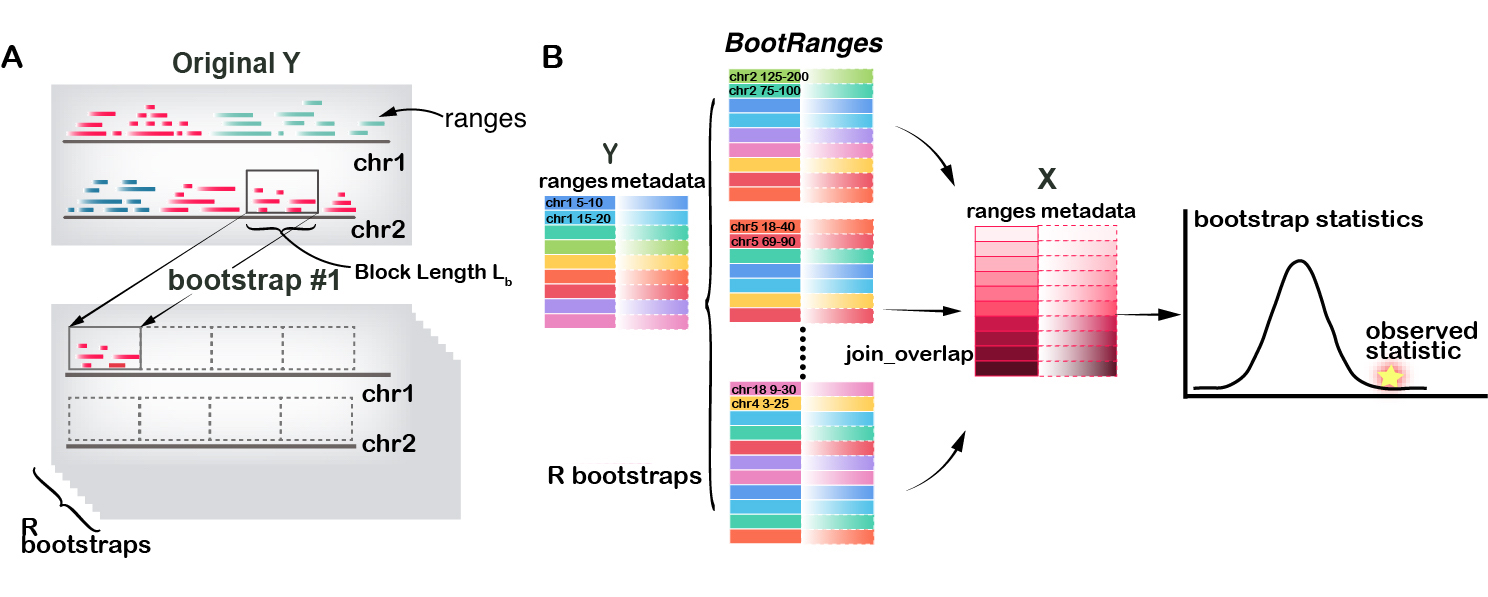
\includegraphics[scale=0.65]{Figures/bootRanges.jpg}
\caption{Schematic overview.
  A) Bootstrapping blocks of length $L_b$ \wancen{from randomly selected position and move to a tile block across chromosome within same states. Each small rectangle represents a feature. Color represents states. Can we say we interchangeably use the terms "ranges” and “features” in the reminder of the paper?} 
  B) \wancen{Workflow of testing null hypothesis of true biological question between \bm{$x$} and \bm{$y$} using \bootranges. Derive \bootranges of \bm{$y$}, calculating the distribution of interested statistics between \bm{$x$} and \bootranges. Permutation test can be performed to access the null hypothesis}} 
\label{fig:framework}
\vspace{-0.5cm}
\end{figure}

\vspace*{-.5cm}
\section{Application}

\wancen{To assess the accuracy of estimating statistics, we compared \bootranges result with shuffling in simulation. Details are in \cref{sec:sim}. We showed that \bootranges can achieve low false positive rate(FPR) as desired. While shuffling generate distribution of statistics with similar mean as original distribution, but smaller variance, therefore the FPR are relatively high and will overestimate how unlikely the observed statistics is.(\cref{fig:simulation}).}


We first applied \bootranges to determine the significance of the
overlap of liver ATAC-seq
\citep{CURRIN20211169} with SNPs associated with total cholesterol,
bootstrapping the SNPs to assess significance.
While the observed overlap was significant across many combinations of
various segmentation methods and $L_b$ according to empirical p-value, 
the variance of the
bootstrap statistics distribution and the resulting $z$ score varied greatly
(\cref{fig:result}A-B).
We used the $z$ score to measure the distance between the observed
statistics and bootstrap distribution in terms of standard deviations.
Overlap rate was defined as the proportion of
SNPs that had peaks within 10kb.
That the variance of the distribution in \cref{fig:result}A for the
unsegmented bootstrap increased with $L_b$ indicated that
ranges are inhomogeneous and
bootstrapping with respect to a genome
segmentation may be a more appropriate choice
\citep{bickel2010subsampling}. 
% inhomogeneous and segmentation could alleviate the scenario.
The decreasing trend using pre-defined segmentation from
Roadmap Epigenomics indicated too many short segments,
where $L_b$ is too close to $L_s$ for effective block randomization.
To choose an optimal segmentation, \wancen{we considered the variance of the bootstrap distribution become stable as $L_b$ increases(\cref{fig:result}A). To choose an optimal $L_b$ range,
two aspects were considered:
provided minimum value of a scaled version of the changes in the variance of test statistic distribution over $L_b$ as recommended previously \citep{bickel2010subsampling},
and the original inter-range distances distribution were preserved (Supplementary \cref{sec:length}).}
Here $L_s \approx 2$ Mb and $L_b \in [300\textrm{kb},600\textrm{kb}]$ was 
shown to be a good range for segment and block
lengths (\cref{fig:suppfig0}A-C, and Supplementary \cref{sec:liveratac}).
The scientific conclusion of this example was that liver ATAC-seq
peaks were
much closer to total cholesterol SNPs than expected even when placing
blocks of SNPs to match a genome segmentation. \wancen{As seen in applications of \citet{bickel2010subsampling}, the effect
of segmentation did not greatly alter conclusions, e.g. rejection of
the null hypothesis, in this case, z score varies from ~4 to ~6 across segmentation choice, though depending on block length. It may vary more in other contexts.}
Shuffling of genomic ranges (Supplementary \cref{sec:shuffle})
resulted in a much higher $z = 18.5$, compared to $z \approx 4$ 
consistent with previous conclusions that shuffling may 
overestimate significance leading to misinterpretation of enrichment.


%\vspace{-0.5cm}
% \newpage
\begin{figure}[H]
\centering% default with `floatrow`
\setlength{\abovecaptionskip}{-0.1cm}
\setlength{\belowcaptionskip}{-0.1cm}
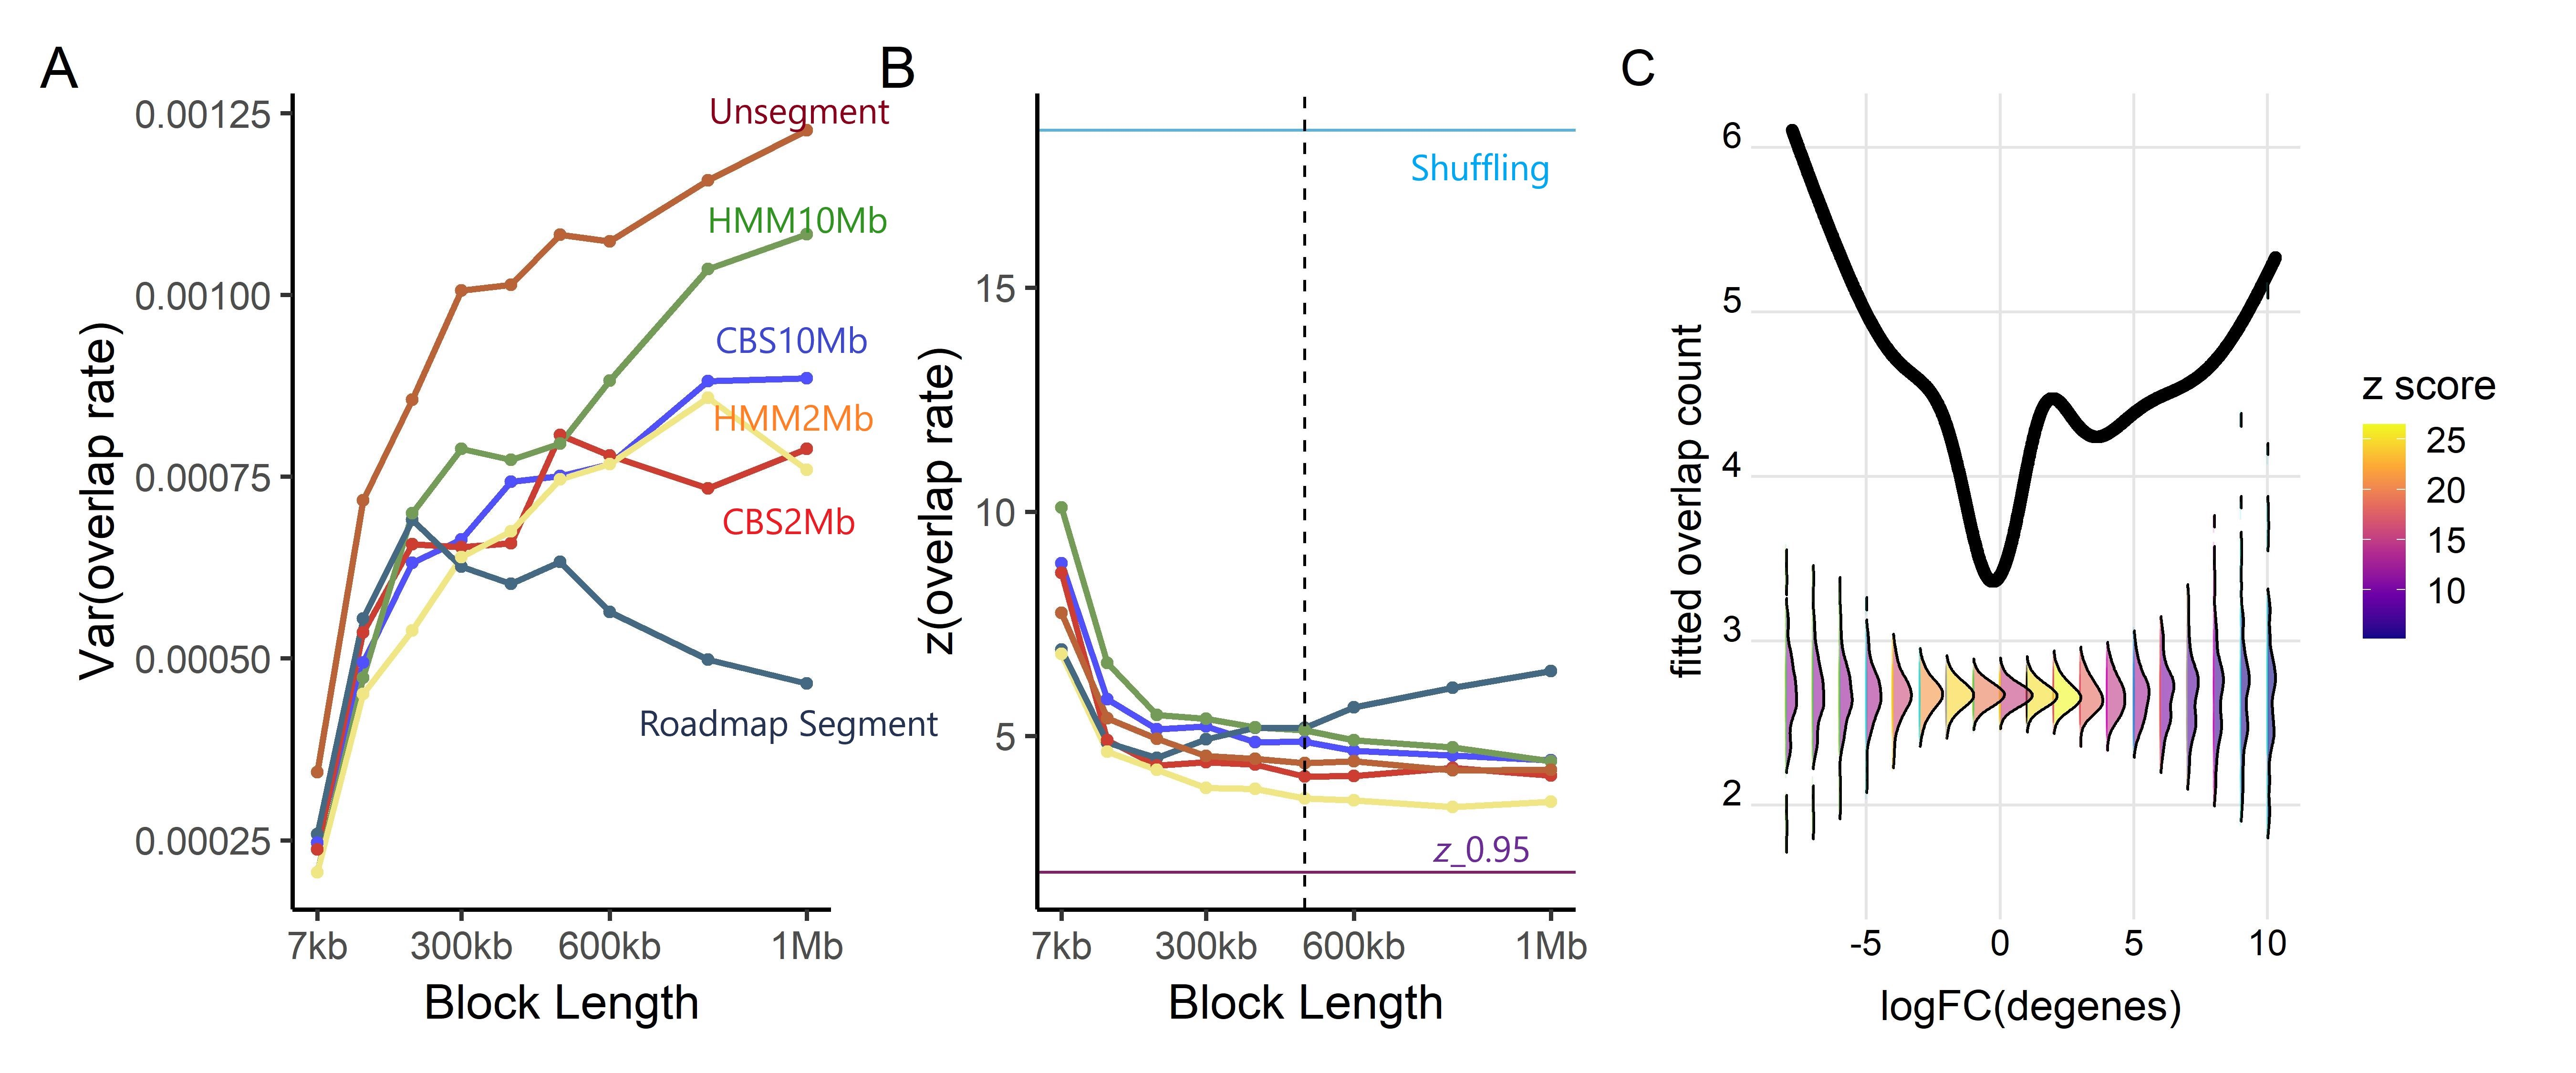
\includegraphics[scale=0.06]{Figures/fig2_3.jpeg}
\caption{
  Parameter selection and overlap analysis.
  A) Variance of the rate of overlaps and,
  B) $z$ score for the overlap,
  for different segmentations and $L_b$ on the liver 
  dataset.
  C) GAM predicted curves for observed (black line) and
  bootstrapped data (densities),
  for the overlap count over gene logFC.
  Conditional densities are colored by the $z$ score for the overlap.
}
\label{fig:result}
\vspace{-.7cm}
\end{figure}

%% z score, independent of number of bootstraps, was used to measure the
%% distance between the expected value and the observed one according to
%% the standard deviations.
%% the $z = 4.10$ if look at circular binary search(CBS)
%% \citep{cbs} segmentation method with $L_s = 2e6$ and
%% $L_b=5e5$(\cref{fig:result}B).
%% As seen in applications of \citet{bickel2010subsampling}, the effect
%% of segmentation did not greatly alter conclusions, e.g. rejection of
%% the null hypothesis, in this case, although the z score varies greatly
%% among the different segmentations and block lengths.

We demonstrated using \bootranges to motivate the choice of data-driven thresholds 
during enrichment analyses. We tested this on a dataset of differential chromatin accessibility and gene expression 
\citep{alasoo2018shared,lee2020fluent} and previous liver ATAC-seq.
A generalized linear model (GLM) with penalized splines was
fit to the overlap count over gene logFC, both for the original
data and to each of the generated null sets.
Conditional densities of splines fit to null sets
were computed at various thresholds to reveal how
the threshold choice would affect the
variance of the bootstrap density and the resulting $z$ score
(\cref{fig:result}C). \wancen{ We show that in fact the observed enrichment with respect to bootstrapped ranges varies over the logFC threshold. Instead of arbitrary logFC cutoff, 
these analyses suggested that SNPs -log10 (\textit{p}-value) $= 8$ and gene expression $|\textrm{logFC}| = 2$ and were optimized thresholds where the $z$ score was highest
(\cref{fig:suppfig2}).}



%We demonstrate using \bootranges to motivate the choice of thresholds 
%that are applied to genomic regions during enrichment analyses.
%We tested this on the aforementioned liver ATAC-seq example, and on a
%dataset of differential chromatin accessibility and gene expression 
%\citep{alasoo2018shared,lee2020fluent}.
%A generalized linear model (GLM) with penalized regression splines was
%fit to the overlap rate or count over the $-\log_{10}(p)$ or
%gene logFC, both for the original
%data and to each of the bootstrap datasets.
%Condition densities of splines fit to bootstrap data
%were computed at various thresholds to reveal how
%the threshold choice would affect the
%variance of the bootstrap density and the resulting $z$ score
%(\cref{fig:result}C-D).
%These analyses suggested that $-\log_{10}(p) = 8$ and
%$|\textrm{logFC}| = 2$
%are optimized thresholds where the $z$ score was highest
%(\cref{fig:suppfig2}A-B).

%We found that the $z$ score was highest when $-\log_{10}(p) = 8$
%(\cref{fig:suppfig2}A),
%and when $\textrm{|logFC|} = 2$(\cref{fig:suppfig2}B).
%(\cref{fig:suppfig2}B).
%% from \textit{gam} function in the
%% \emph{mgcv} R package were fitted and \textit{predict\_gam} function
%% in the \emph{tidymv} R package were predicted on observed and each
%% null sets.
%% $$
%% \setlength{\abovedisplayskip}{3pt}
%% \setlength{\belowdisplayskip}{3pt}
%% log \left( \frac{\pi}{1-\pi} \right) = \beta_0  + f (-log_{10}p), log(\mu) = \beta_0 + f (log_{FC})
%% $$ 
%% for rate and count-based statistic, separately.
%% All generated 95\%
%% percentile intervals at the same time across a range of effect sizes
%% were displayed by conditional density plot 

We applied \bootranges to
%Chromium Single Cell Multiome
single cell multiome
ATAC-seq and RNA-seq, to assess the correlation ($\rho$) of log counts for the two
modalities for all pairs of genes and peaks, across
14 cell types (pseudo-bulk). Across all genes, we observed
$\bar{\rho} = 0.33$, which was 
significantly higher than the bootstrap correlation mean
(\cref{fig:suppfig3}A, $\bar{\rho}_{R} = 0.007$). As expected, RNA
and ATAC measured at local peaks had similar cell-type-specificity.
Additionally, the average gene-peaks correlation per gene can be
computed and compared to a bootstrap distribution to
identify gene-promoter pairs that were significantly correlated across
cell types (\cref{fig:suppfig3}B-C).


To compare speed, we ran \bootranges and GSC on
ENCODE kidney and bladder ChIP-seq. The average time to
block bootstrap the genome using \bootranges was 0.30s and
0.37s with overlap computation. A comparable analysis with GSC took
7.56s.


\vspace*{-20pt}
\section{Conclusion}

\bootranges efficiently generates null models of genomic ranges preserving 
local genomic correlations, and can be used easily in combination with
other range-based tools such as \plyranges.
It has great flexibility in various disciplines (e.g. identify
putative transcription factor binding site according to enriched peak
regions).

% All of the R code and data used in this paper are available at the
% following repository: 
% \url{https://github.com/Wancen/bootRangespaper}.

\vspace*{-20pt}

\section*{Funding}
CZI EOSS and R01-HG009937 to M.I.L, NIH R35-GM128645 to D.H.P.

\vspace*{-20pt}


% \vspace*{-15pt}


\bibliographystyle{natbib}
%\bibliographystyle{achemnat}
%\bibliographystyle{plainnat}
%\bibliographystyle{abbrv}
%\bibliographystyle{bioinformatics}
%
%\bibliographystyle{plain}
%
\bibliography{document}
\end{document}
